\documentclass{article}
\usepackage{graphicx} % Required for inserting images
\usepackage[export]{adjustbox}
\usepackage{listings}
\usepackage{color}
\usepackage{tabularray}

\definecolor{dkgreen}{rgb}{0,0.6,0}
\definecolor{gray}{rgb}{0.5,0.5,0.5}
\definecolor{mauve}{rgb}{0.58,0,0.82}

\lstset{
frame=tb,
language=C,
aboveskip=3mm,
belowskip=3mm,
showstringspaces=false,
columns=flexible,
basicstyle={\small\ttfamily},
numbers=none,
numberstyle=\tiny\color{gray},
keywordstyle=\color{blue},
commentstyle=\color{dkgreen},
stringstyle=\color{mauve},
breaklines=true,
breakatwhitespace=true,
tabsize=3
}

\title{Algoritmo parallelo per la somma di N numeri}
\author{Puggioni Riccardo,Regina Riccardo,Trotti Francesco }
\date{October 2023}

\begin{document}

\maketitle

\section{Introduzione al problema}
\subsection{Somma di N numeri}
    L'algoritmo per la somma di N numeri fa parte di quei problemi
    il cui approccio alla risoluzione è detto di "riduzione".
    Parallelizzare Questo tipo di algoritmi può essere particolarmente insidioso:
    quando si sommano N numeri quello che si fa è eseguire N-1
    operazioni di somma; il nostro obiettivo è cercare di parallelizzare le operazioni di somma eseguendole su più processori diversi diminuendo in questo modo i passi temporali necessari alla risoluzione del problema.

    Ciò che però ci preme è non solo di risolvere il problema
    dato utilizzando un algoritmo parallelo, ma cercare di sfruttare al meglio il nostro ambiente di calcolo.
\subsection{Approccio alla risoluzione del problema dato}

   

    Andiamo dunque ad implementare la strategia di parallelizzazione in linguaggio C utilizzando una libreria per il "message passing" in un sistema MIMD (la libreria MPI).
    \\
    L'idea principale per la risoluzione del problema è di dividere l' array fra i vari processori.
    Fatto questo, ogni processore dovrà calcolare la somma parziale degli elementi del suo sotto-array
    e si dovranno poi ricostruire le varie somme parziali in maniera opportuna per ottenere la soluzione finale.\\
    \begin{figure}[!htbp]
        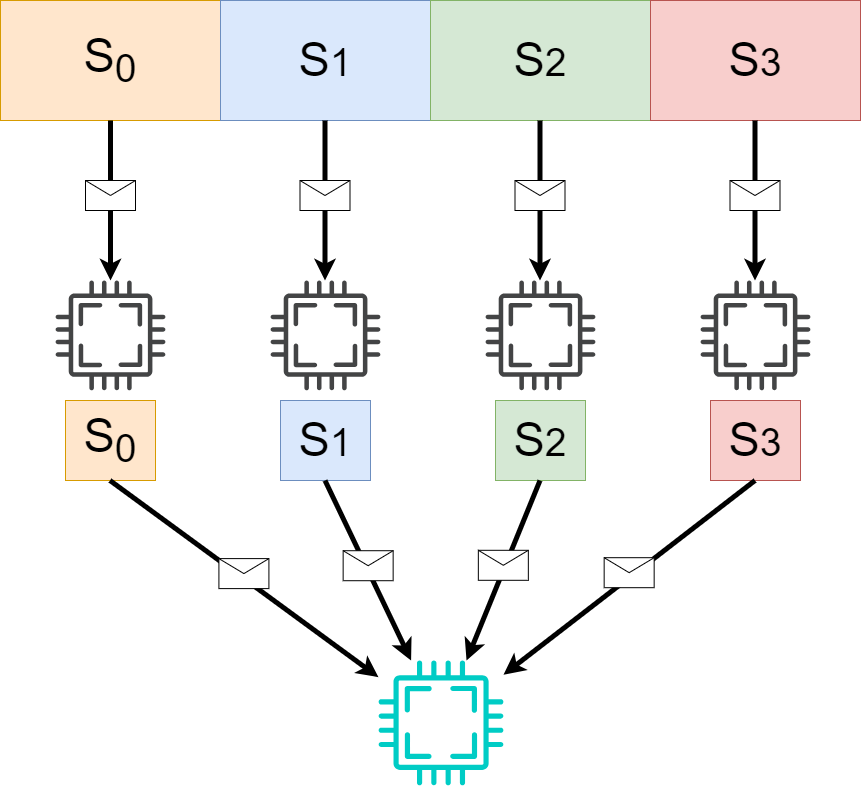
\includegraphics[width=0.3\linewidth,center]{divisione_array.drawio.png}
        \caption{Divisione dell array in parti}
        \label{fig:enter-label}
    \end{figure}  
    
    Ipotizziamo ora di voler implementare il nostro algoritmo, individuiamo tre passi fondamentali:
    \begin{enumerate}
        \item dividiamo l'array in più parti e assegnamo ogni parte a un processore.
        \item ogni processore esegue la propria somma parziale.
        \item si ricombinano le soluzioni parziali e si ottiene la soluzione finale.
    \end{enumerate}

    Facendo in questo modo possiamo così eseguire più somme concorrentemente, e il nostro algoritmo sarà di conseguenza più rapido.\\
    Una prima idea sarebbe dunque quella di prendere la dimensione dell array e di dividerla per il numero dei processori utilizzati: in questo modo otteniamo (all'incirca) il numero di elementi che ogni sotto-array dovrà contenere (a meno dei resti della divisione che si dovranno poi gestire nell'implementazione).

    \begin{figure}[!htbp]
        \centering
        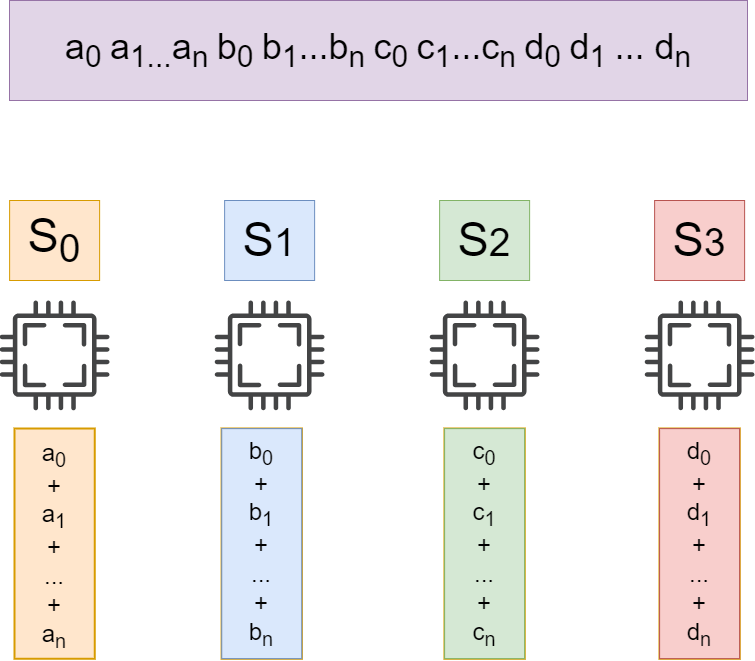
\includegraphics[width=0.6\linewidth]{somme_parziali.drawio (1).png}
        \caption{Ogni processore esegue la sua somma}
        \label{fig:enter-label}
    \end{figure}

    Una volta eseguita la distribuzione dei dati fra i vari processori passiamo all' algoritmo vero e proprio: ogni processore non deve far altro che sommare gli elementi del proprio sotto-array producendo le somme parziali.\\
    

\subsection{Strategie di comunicazione}
 Bisogna ora capire il modo in cui queste somme devono essere ricombinate, a tal scopo analizziamo tre possibili modalità di procedere:
\subsubsection{Strategia I}
    La prima strategia è la più intuitiva.
    Consiste nel prendere le varie somme parziali e mandarle tutte ad un processore specifico: sarà lui che eseguirà la somma delle varie somme parziali e che otterrà la soluzione finale al problema.
    Tuttavia seppur questa implementazione sia molto semplice (e funzionante in ogni caso), non rappresenta sempre la scelta più performante in quanto una volta che inviamo al processore scelto tutte le somme parziali, questo eseguirà la somme rimanenti in maniera sequenziale, mentre gli altri processori non saranno utilizzati affatto. La somma finale sarà presente dunque soltanto nella memoria del processore scelto per il calcolo finale.\\
    Come si evince anche dalla figura, ci saranno delle somme che potevano essere parallelizzate ulteriormente...(in date condizioni). 

    \begin{figure}
        \centering
        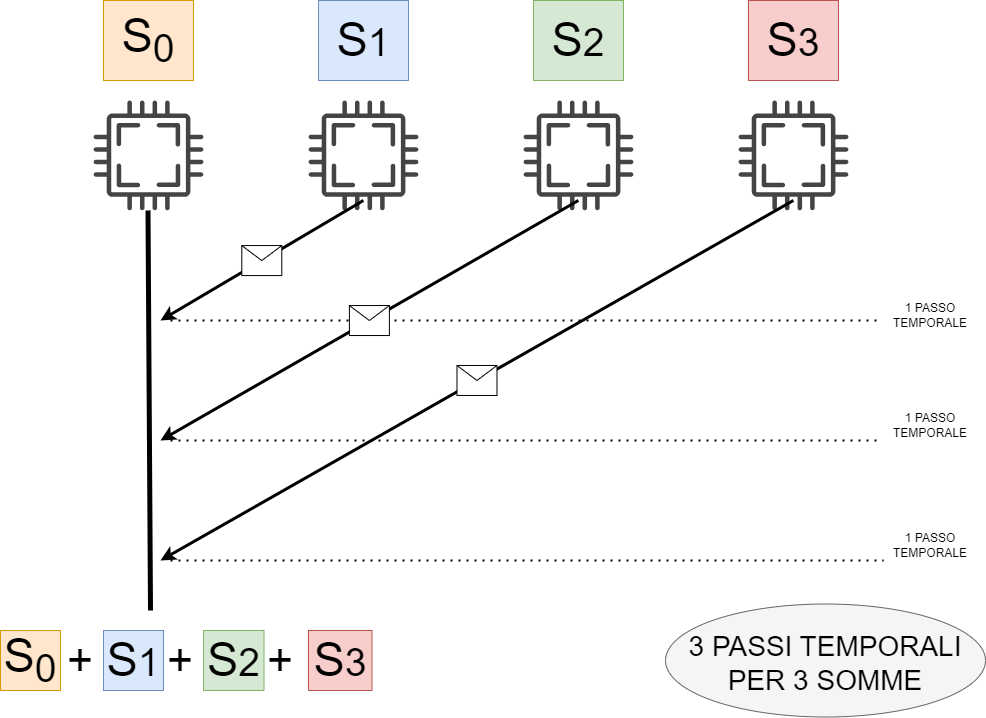
\includegraphics[width=1\linewidth]{strategia_I.drawio.png}
        \caption{Ognuno invia ad un processore}
        \label{fig:enter-label}
    \end{figure}
\subsubsection{Strategia II}
    La seconda strategia differisce dalla prima poichè i processori si dividono in coppie: uno dei due invia all'altro la propria somma parziale e l'altro ricevendo i dati aggiorna la propria somma.
    Alla fine l'ultima coppia aggiornerà l'ultima somma parziale ottenendo il risultato finale.
    L'ultimo processore che riceverà conterrà la somma totale.\\
    Tuttavia ci accorgiamo subito che, in una prima analisi preliminare, l'implementazione di questa strategia fa sicuramente sì che si risparmino passi temporali preziosi, ma può essere applicata soltanto se il numero dei processori in gioco è una potenza di due. Infatti non potrei dividere i processori sempre in coppie se questa condizione non fosse soddisfatta.
\begin{figure}
    \centering
    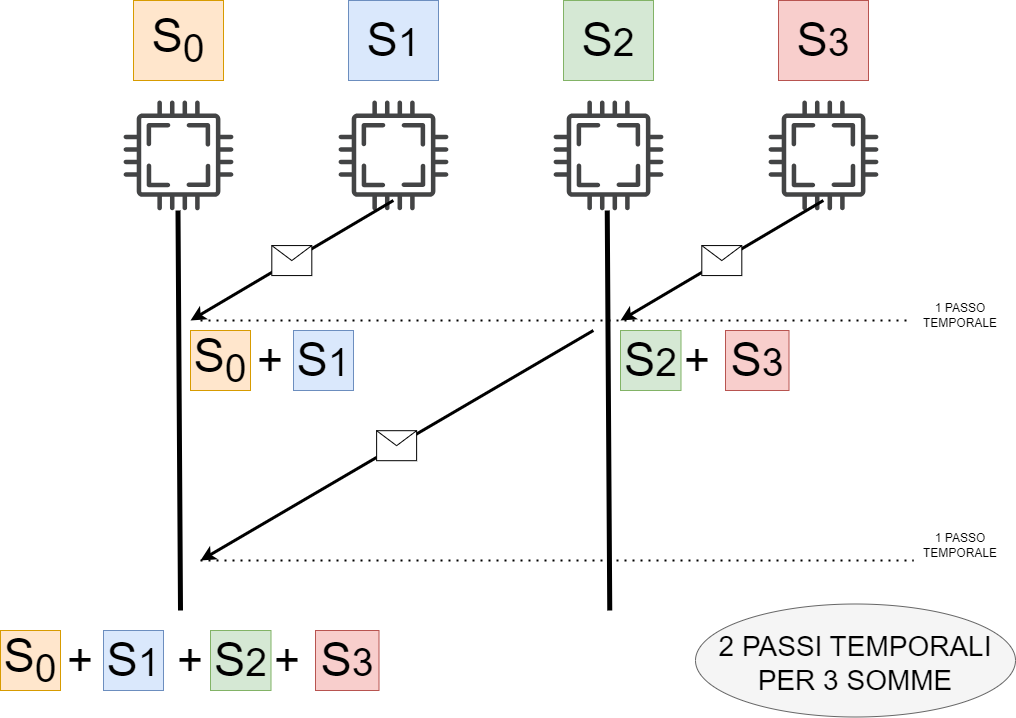
\includegraphics[width=1\linewidth]{strategia_II.drawio.png}
    \caption{In coppie (uno manda e uno riceve)}
    \label{fig:enter-label}
\end{figure}
\subsubsection{Strategia III}
    La terza strategia è simile alla seconda: divido sempre in processori in coppia.
    Tuttavia questa volta ogni coppia di processori si invia a vicenda la propria somma parziale e aggiornano entrambi la loro somma. Alla fine saranno tutti i processori ad avere il risultato finale in memoria.Tuttavia i passi temporali che risparmiamo sono gli stessi della strategia due, la principale differenza è infatti nel solo fatto che tutti i processori alla fine avranno la somma totale.
    \begin{figure}[!h tbp]
        \centering
        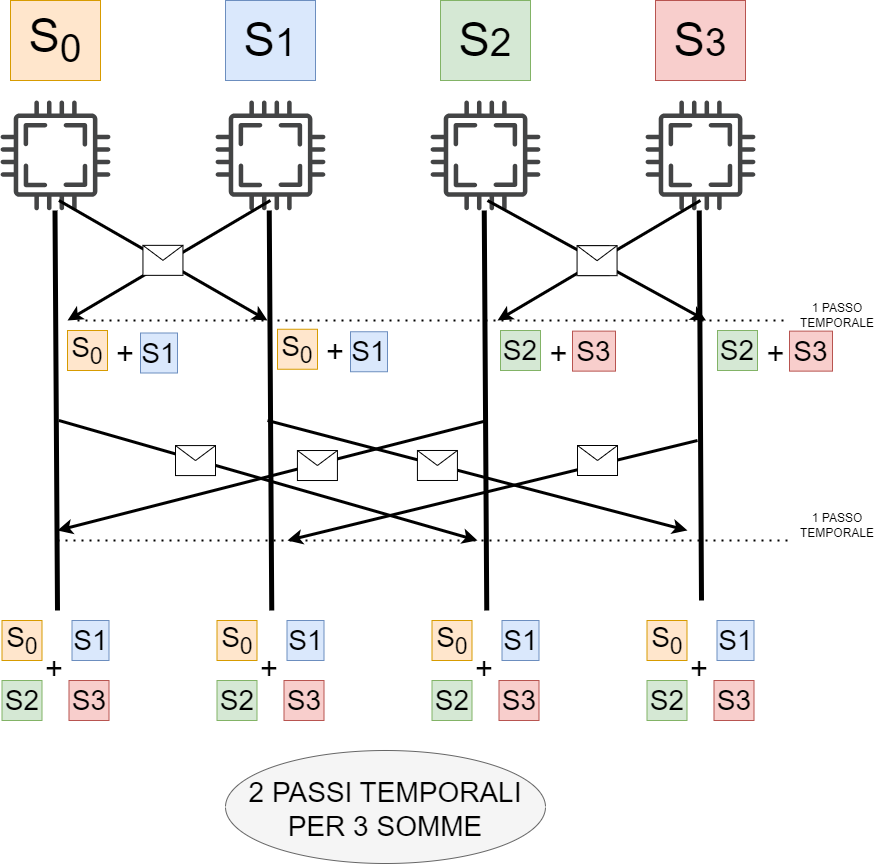
\includegraphics[width=1\linewidth]{strategia_III.drawio.png}
        \caption{In coppie (entrambi mandano e ricevono)}
        \label{fig:enter-label}
    \end{figure}
\clearpage
\section{Implementazione dell'algoritmo}
\subsection{Header file richiamati}
\begin{lstlisting}
#include <stdlib.h>
#include <stdio.h>
#include <math.h>
#include "mpi.h"
\end{lstlisting}

\subsection{Implementazione}
\begin{lstlisting}


#define BAD_STRATEGY_VALUE 10
#define BAD_ARRAY_SIZE 20
#define ERRORE_ALLOCAZIONE_MEMORIA 30
void gestisciErrore(int error_code);
int isPowerOf2(int x);

int main(int argc,char *argv[])
{    
    /*
        1) lettura di strategia
        2) inizio delle comunicazioni MPI
        3) Decido se la strategia e' applicabile
        4) leggo i dati da file
        5) allineo i processi
        6) ogni processore esegue le somme parziali
        7) applico una strategia di comunicazione
        8) chiudo le comunicazioni MPI
        9) stampo il risultato con un solo processo
    */

    int pid, n_processi; //pid è il process id, n_processi è il numero di processi
    int strategy; //la strategia specificata dall'utente
    int *array; //array che conterrà i numeri letti da file
    int dim; // dimensione di array
    int *array_locale, start, dim_locale; //il sottoarray di competenza di un processo
    //start è l'indirizzo del primo elemento di un sottoarray
    //dim_locale è la dimensione del sottoarray
    int rest; //gli elementi in esubero da ridistribuire equamente ai processi
    int tag; //tag è l'identificativo di una comunicazione tra due processi
    double tempo_tot; //tempo totale serve al processo 0 per calcolare il massimo fra tutti i tempi di esecuzione
    double t_0; // serve ad ogni processo per prendere il tempo iniziale
    double t_1; // serve ad ogni processo per prendere il tempo finale
    double time; // serve ad ogni processo per calcolare t_1 - t_0
    MPI_Status status; //indica lo stato di una comunicazione

    MPI_Init(&argc, &argv); //Inizio delle comunicazioni

    strategy = atoi(argv[1]);
    if(pid==0)printf("strategy before--->%d",strategy);
    if (strategy != 1 && strategy != 2 && strategy != 3) {
        gestisciErrore(BAD_STRATEGY_VALUE);
        strategy = 1;
        //continuo lo stesso con la strategia 1
    }


    MPI_Comm_rank(MPI_COMM_WORLD, &pid); //ogni processo inserisce il proprio identificativo nella variabile pid. 
    MPI_Comm_size(MPI_COMM_WORLD, &n_processi); //Ogni processo viene a conoscenza del numero di processi.

    //Decido la strategia
    int potenzaDi2 = isPowerOf2(n_processi);
    //se strategy = 2,3 AND n_processi non è potenza di 2 ALLORA procedo con la strategia 1. 
    if (potenzaDi2 == 0 && (strategy == 2 || strategy == 3)) {
        printf("Strategie 1, 2 non applicabili: procedo con la strategia 1\n");
        strategy = 1;
    }

    if (pid==0) {
        //leggi i dati dall input (n e x)
        FILE *fp;
        fp = fopen("/homes/DMA/PDC/2024/<LOGIN>/sum/sum.txt","r"); //e' richiesto il PATH intero

        fscanf(fp,"%d ",&dim);
        if (dim < n_processi || dim < 0) {
            gestisciErrore(BAD_ARRAY_SIZE);
            exit(1);
        }

        array = malloc(dim*sizeof(int));
        if (array == NULL) {
            gestisciErrore(ERRORE_ALLOCAZIONE_MEMORIA);
            exit(1);
        }
        
        int i;
        for (i = 0; i < dim; i++){
            fscanf(fp,"%d ",&array[i]);
        }
        
        fclose(fp);
    }

    MPI_Bcast(&dim, 1, MPI_INT, 0, MPI_COMM_WORLD); //ogni processo ottiene la dimensione dell array di input (i processi si sincronizzano).

    dim_locale = dim / n_processi; //dividiamo la dimensione dell array per il numero di processi 
    rest = dim % n_processi;     //e gestiamo il resto in modo da ottenere la dimensione
    if (pid < rest) {           // del sottoarray per ogni processo.
        dim_locale++;
    }

    int tmp;
    if (pid==0) {
        array_locale = array;
        tmp = dim_locale;
        start = 0;
        int i;
	    for (i = 1; i < n_processi; i++){    //spezziamo l array in piu parti e mandiamo
            start = start + tmp;              //ad ogni processo la sua parte.
            tag = 22 + i;
            if (i == rest) {	
                tmp--;
		    }
            MPI_Send(&array[start], tmp, MPI_INT, i, tag, MPI_COMM_WORLD);
        }
    }
    else
    {
        tag = 22 + pid;
        array_locale = malloc(dim_locale*sizeof(int));
	    MPI_Recv(array_locale, dim_locale, MPI_INT, 0, tag, MPI_COMM_WORLD, &status);  
        //i processi ricevono la propria parte.
    }


    MPI_Barrier(MPI_COMM_WORLD); //sincronizzo i processi in modo che tutti partano dallo stesso istante. (kekko: ipotizzo che funzioni anche senza ma vabbe)
    t_0=MPI_Wtime(); // tutti i processi prendono l'istante iniziale t_0.


    //--------------------------------------
    //inizio dell'algoritmo vero e proprio.
    //--------------------------------------

    //tutti i processori eseguono la propria somma parziale:
    int somma_parziale;
    int i;
    int sum=0;
	for (i = 0; i<dim_locale; i++) {
       	sum = sum + array_locale[i];
	}
    printf("sono %d e la mia somma parziale--->%d\n",pid,sum);

    int somma_totale = 0;
    //Strategia di comunicazione
    if(pid==0)printf("eseguo startegia:%d\n",strategy);
    if (strategy == 1) {
        if (pid == 0){
            for (i = 1; i < n_processi; i++){
                tag = 69 + i;
                MPI_Recv(&somma_parziale, 1, MPI_INT, i, tag, MPI_COMM_WORLD, &status);
                sum = sum + somma_parziale;
            }
        }
        else
        {
            tag = 69 + pid;
            MPI_Send(&sum, 1, MPI_INT, 0, tag, MPI_COMM_WORLD);
        }
    }
    else if (strategy == 2) {
        for (i = 0; i < log2(n_processi); i++) {
            if (pid % (int)pow(2,i) == 0) {
                if (pid % (int)pow(2,i+1) == 0) {
                    tag = pid;
                    MPI_Recv(&somma_parziale, 1, MPI_INT, pid+pow(2,i), tag, MPI_COMM_WORLD, &status);
		    sum = sum + somma_parziale;
                } 
                else
                {
                    tag = abs(pow(2,i) - pid);
                    MPI_Send(&sum, 1, MPI_INT, tag, tag, MPI_COMM_WORLD);
                }
            }
        }
    }
    else if(strategy == 3){
        for (i = 0; i < log2(n_processi); i++) {
            int mod = pow(2,i+1);
            if (pid % mod < pow(2,i)) {
                tag = pid;
                MPI_Send(&sum, 1, MPI_INT, pid+pow(2,i), tag, MPI_COMM_WORLD);
                MPI_Recv(&somma_parziale, 1, MPI_INT, pid+pow(2,i), tag, MPI_COMM_WORLD, &status);
            } else {
                tag = pid - pow(2,i);
                MPI_Send(&sum, 1, MPI_INT, pid-pow(2,i), tag, MPI_COMM_WORLD);
                MPI_Recv(&somma_parziale, 1, MPI_INT, pid-pow(2,i), tag, MPI_COMM_WORLD, &status);
            }
            sum=sum+somma_parziale; //la somma la faccio comunque
        }
    }

    t_1=MPI_Wtime();//tutti i processi prendono il tempo finale.

    time= t_1 - t_0;//ogni processo calcola il proprio tempo.
    printf("sono il processo %d, tempo impiegato:%e\n",pid,time);
    
    MPI_Reduce(&time,&tempo_tot,1,MPI_DOUBLE,MPI_MAX,0,MPI_COMM_WORLD);  // utilizziamo la reduce sui vari tempi per ottenere il massimo (contenuto dal processo 0).

    //Stampo la somma e il tempo totale di esecuzione con il processo con pid 0.
    if(pid==0){
	FILE *fp;
	fp=fopen("/homes/DMA/PDC/2024/<LOGIN>/sum/tempi.txt","a");
	fprintf(fp,"dimensione=%d processori=%d strategia=%d\n",dim,n_processi,strategy);
        fprintf(fp,"somma=%d\n",sum);
        fprintf(fp,"tempo totale di esecuzione--->%e\n\n\n",tempo_tot);
	fclose(fp);
    }

    //Fine delle istruzioni MPI
    MPI_Finalize();

}

void gestisciErrore(int error_code)
{   
    FILE* fp = fopen("/homes/DMA/PDC/2024/RGNRCR04F/sum/sum.err","a")
    if (error_code == BAD_STRATEGY_VALUE) {
        //Stampo nel file di errori l'errore trovato.
        fprintf(fp, "Errore nell'inserimento di 'strategy'.\n");
    }
    else
    if (error_code == BAD_ARRAY_SIZE) {
        fprintf(fp, "Errore nell'inserimento di 'dim'.\n");
    }
    else
    if (error_code == ERRORE_ALLOCAZIONE_MEMORIA) {
        fprintf(fp, "Errore di allocazione in memoria.\n");
    }
}

int isPowerOf2(int x)
{
    return (x != 0) && ((x & (x - 1)) == 0);
}
\end{lstlisting}

\section{Analisi dei tempi di esecuzione}
\subsection{Tempo di esecuzione}

Nell' approccio a calcolare il tempo di esecuzione di un algoritmo parallelo, la grandezza nota come complessità di tempo (utile nell analisi del tempo di esecuzione di un algoritmo sequenziale) diventa inutilizzabile.\\
In un algoritmo parallelo il numero delle operazioni non coincide più con il numero dei passi temporali, di conseguenza si introducono nuove grandezze al fine di realizzare un analisi degli algoritmi paralleli. Nel caso particolare in cui si debbano sommare N numeri, il numero di operazioni di somma da effettuare è N-1.

In un ambiente di calcolo parallelo con P che indica il numero di processori, un problema che si risolve in un tempo T ci darà che, \textit{T(P)} è il \textit{tempo di esecuzione su p processori}. Il problema si svolgerà (idealmente) in $$ \frac{T}{P}. $$ \\


\subsection{Speed-up, Overhead ed Efficienza}

Lo \textbf{Speed- up} misura la riduzione del tempo di esecuzione rispetto all'algoritmo su 1 processore ed è definito dal rapporto:
$$ S(P) = \frac{T(1)}{T(P)} $$ 


La quantità che misura di quanto il nostro speed up differisce da quello ideale è l'overhead. Si può quantificare con la seguente formula: $O_h(p) = pT(p) - T(1)$ .\\
Riscrivendo lo speed up in funzione dell overhead ci accogiamo infatti che lo speed up è ideale se e solo se l'overhead è 0.\\


Lo speed-up che noi vogliamo ottenere è uno speed up il più prossimo possibile a quello che si definisce come speed-up ideale (che si ottiene con S(P) = P).

Per poter misurare se e quanto è stato "sfruttato" il nostro ambiente di calcolo parallelo dobbiamo calcolare l' \underline{efficienza} del nostro algoritmo.
Si definisce \textbf{efficienza} il rapporto: $$ E(p) = \frac{S(p)}{p} $$\\

\subsection{Speed Up scalato e isoefficienza}
Sebbene abbiamo ora delle grandezze per misurare i tempi di esecuzione di un algoritmo parallelo (speed up ed efficienza),
ci chiediamo se sia possibile ottenere speed up prossimi a quello ideale.\\
Dobbiamo a tal fine inserire il concetto di \textbf{scalabilità}.
Tutto parte dal concetto di dividere un algoritmo in due parti:
\begin{enumerate}
    \item $$\alpha$$ è la parte che può essere eseguita esclusivamente in maniera sequenziale.
    \item $$1-\alpha$$ è la parte che può essere parallelizzata fra più processori.
\end{enumerate}
Individuando queste due componenti principali possiamo arrivare a formulare un nuovo modello di speed up:

$$S(p)=\frac{1}{\alpha-\frac{(1-\alpha)}{p}}$$

Questa legge ,nota come \textbf{legge di Ware}, ci permette di osservare cosa succede quando variamo assieme la dimensione del problema e il numero di processori.
La soluzione ottimale per ottenere uno speed up vicino a quello ideale e, in contemporanea, una buona efficienza che \underline{non degrada}, dobbiamo far variare in contemporanea sia il numero dei processori che la dimensione del problema.
Arriviamo così al concetto di speed up scalato:
$$SS(p,n)=\frac{T(1,pn)}{T(p,pn)}=\frac{pT(1,n)}{T(p,pn)}$$

Ma di quanto deve aumentare la dimensione del problema in proporzione al numero dei processori?\\
Introduciamo, per questo motivo, una funzione che calcola esattamente questo coefficiente, la funzione isoefficienza: 
$$I(n_{0}, p_{0}, p_{1}) = n_0\frac{p_{1} log_{2} p_{1}}{p_{0} log_{2} p_{0}} = n_1$$
Osserviamo inoltre che:
\begin{enumerate}
    \item Se aumentiamo p e teniamo n fissato allora le prestazioni peggiorano!.
    \item Se aumentiamo n e teniamo p fissato allora lo speed up si avvicina sempre di piu a quello ideale (ma non possiamo aumentare arbitrariamente la dimensione del problema con un hardware limitato...).
    \item Se aumentiamo n proporzionalmente a p secondo un coefficiente ricavato dall isoefficienza, allora otteniamo speed up vicino a quello ideale e l'efficienza rimane (bene o male) costante. (migliore soluzione)
\end{enumerate}
Grazie a questi nuovi concetti possiamo finalmente tentare di ottenere speed up (scalati) tendenti allo speed up ideale.
\subsection{Dati empirici}
L'algoritmo è stato testato in più condizioni e secondo i parametri precedentemente descritti.

Avendo fissato ad un milione la dimensione del problema ed avendo fatto variare il numero di processori da 1 a 8, tenendo conto esclusivamente delle potenze di 2, sono stati ottenuti i seguenti risultati:

\begin{table}[htp]
\centering
\caption{Strategia 1}
\begin{tblr}{
  hlines,
  vlines,
}
Processori & Speed Up & Efficienza & Overhead ( * 10\^{}-3 s) \\
2          & 1.84     & 0.92       & 0.34                     \\
4          & 3.45     & 0.86       & 0.62                     \\
8          & 6.3      & 0.79       & 1.04                     
\end{tblr}
\end{table}

\begin{table}[htp]
\centering
\caption{Strategia 2}
\begin{tblr}{
  hlines,
  vlines,
}
Processori & Speed Up & Efficienza & Overhead ( * 10\^{}-3 s) \\
2          & 1.87     & 0.93       & 0.26                     \\
4          & 3.57     & 0.86       & 0.46                     \\
8          & 6.41     & 0.80       & 0.94                     
\end{tblr}
\end{table}

\begin{table}[htp]
\centering
\caption{Strategia 3}
\begin{tblr}{
  hlines,
  vlines,
}
Processori & Speed Up & Efficienza & Overhead ( * 10\^{}-3 s) \\
2          & 1.68     & 0.84       & 0.72                     \\
4          & 3.27     & 0.82       & 0.86                     \\
8          & 6.10     & 0.76       & 1.18                     
\end{tblr}
\end{table}

\clearpage

Visualizziamo la curva, confrontandola all'andamento dello speed-up ideale:
\begin{figure}[h!tbp]
    \centering
    \includegraphics[width=1\linewidth]{WhatsApp Image 2023-10-23 at 21.20.23.jpeg}
    \caption{Andamento degli Speed Up}
    \label{fig:enter-label}
\end{figure}
\clearpage
Visualizziamo su un grafico anche i valori degli Overhead ottenuti per ogni strategia:

\begin{figure}[h!tbp]
    \centering
    \includegraphics[width=1\linewidth]{WhatsApp Image 2023-10-23 at 21.20.23 (2).jpeg}
    \caption{Andamento degli Overhead}
    \label{fig:enter-label}
\end{figure}

\clearpage

Infine osserviamo come varia la nostra efficienza:
\begin{figure}[h!tbp]
    \centering
    \includegraphics[width=1\linewidth]{WhatsApp Image 2023-10-23 at 21.20.23 (1).jpeg}
    \caption{Andamento dell' efficienza}
    \label{fig:enter-label}
\end{figure}

Per non far degradare lo speedup, possiamo sfruttare il concetto di isoefficienza: per sfruttare l'aumento di processori, dobbiamo aumentare anche la dimensione del problema. Il coefficiente di aumento della dimensione non è costante, ma va opportunamente calcolato. Nel nostro caso, l'isoefficienza è la seguente:
$$I(n_{0}, p_{0}, p_{1}) = n_0\frac{p_{1} log_{2} p_{1}}{p_{0} log_{2} p_{0}} = n_1$$
dove $n_0$ è la dimensione del problema per $p_0$ processori, $n_1$ è la dimensione che vogliamo calcolare per $p_1$ processori.

\end{document}

\end{document}
